% NeuroCam manual - Repository Data
% Written by Christopher Thomas.
% Copyright (c) 2021 by Vanderbilt University. This work is released under
% the Creative Commons Attribution-ShareAlike 4.0 International License.

\chapter{Repository Data}
\label{repo}

NeuroCam session data is stored in a ``repository''. Each session has its
own timestamped repository folder, containing some or all of the following:

\begin{itemize}

\item Raw video capture frames, stored as JPEG images in the ``Scene''
and ``Face'' folders.
\item Raw game capture frames, stored as JPEG images in the ``Game'' folder.

\item A ``Monitor'' folder containing reduced-size composited frames that
were sent to the monitoring GUI during the experiment. The composited frames
are not necessarily synchronized with each other.

\item A ``Composite'' folder containing larger composited frames produced
during post-processing. These composited frames should be synchronized.

\item A ``\verb+session.cfg+'' file containing information about the
settings used for the capture session. This file is described in detail in
Chapter \ref{structs}.

\item A ``\verb+logfile.txt+'' file containing raw event data (frame times,
user-supplied markers, and so forth).

\item Post-processed log files ``\verb+logfile-timed.txt+'' and
``\verb+logfile-composited.txt+''. The ``\verb+-timed+'' file has properly
synchronized timestamps and the ``\verb+-composited+'' file includes
timestamps for the ``Composite'' video stream (properly synchronized).

\item Several ``\verb+.mp4+'' compressed video files corresponding to the
video frame folders described above. These are lower-fidelity copies intended
to simplify review of footage.

\end{itemize}

% FIXME - Force a page break.
\clearpage
A typical session folder before post-processing is shown below:
\begin{center}
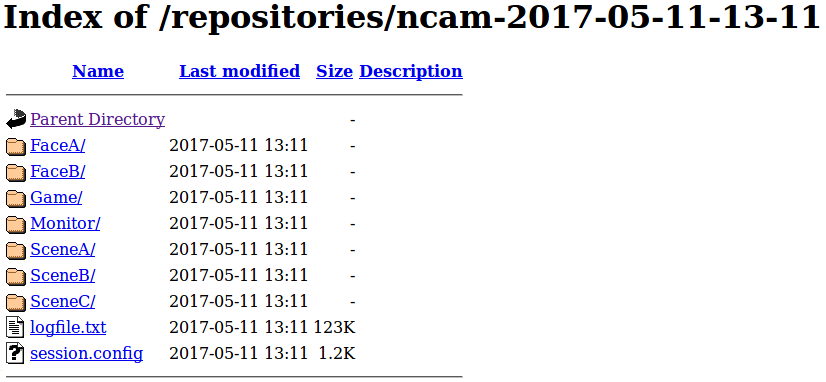
\includegraphics[width=0.6\textwidth]{pics-gui/gui-repo-unprocessed.png}
\end{center}

A typical session folder after post-processing is shown below:
\begin{center}
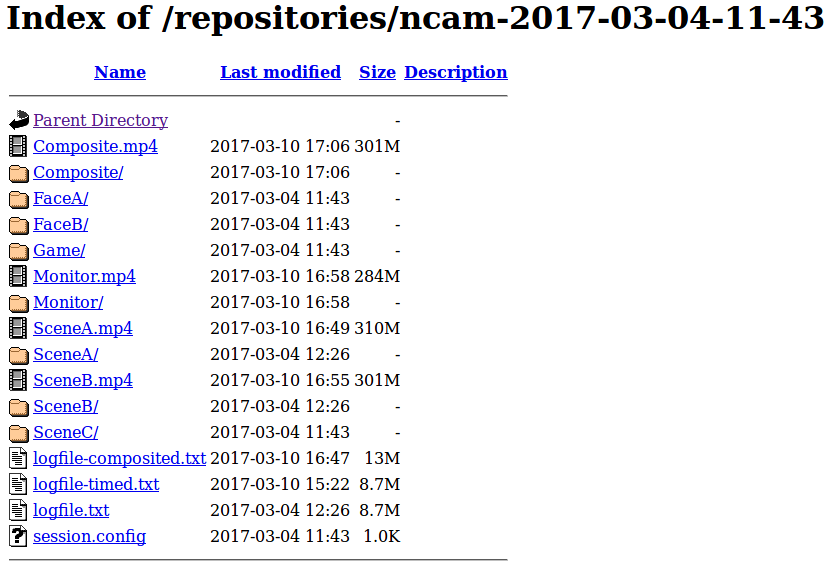
\includegraphics[width=0.6\textwidth]{pics-gui/gui-repo-afterprocess.png}
\end{center}

% FIXME - Force a page break.
\clearpage
\section{Log File Format}

The logfile is a human-readable text file recording one event per line. The 
following types of event are recorded:
\begin{itemize}
\item \textbf{Frame events}, indicating that a video frame was recorded.
This may be from a camera, from a remote computer video feed, or from a
generated feed like the ``Monitor'' and ``Composite'' feeds.
\item \textbf{Network message events}, which are typically sent by the
GPIO-and-synch box or by external applications such as the game.
\item \textbf{Local GUI events}, which are either user annotations, user
markers, or instructions to change the monitoring display.
\end{itemize}

\textbf{Frame events} indicate arrival time, stream ``slot'' name, sequence 
number, and the filename (including subfolder) where the frame was saved. 
Typical frame events are as follows:
\begin{verbatim}
(1367) [SceneA]  frame 8  SceneA/00000008.jpg
(1374) [SceneB]  frame 16  SceneB/00000016.jpg
(1382) [Monitor]  frame 36  Monitor/00000036.jpg
(1403) [SceneB]  frame 17  SceneB/00000017.jpg
(1417) [Monitor]  frame 37  Monitor/00000037.jpg
(1437) [SceneA]  frame 9  SceneA/00000009.jpg
(1444) [SceneB]  frame 18  SceneB/00000018.jpg
\end{verbatim}

\textbf{Netowrk events} indicate arrival time, IP and port of the source,
and a message string. Typical network events are as follows:
\begin{verbatim}
(304) [192.168.1.101:8888]  MSG Unity timestamp 53284 ms
(1303) [192.168.1.101:8888]  MSG Unity timestamp 54283 ms
(2303) [192.168.1.101:8888]  MSG Unity timestamp 55283 ms
(2795) [192.168.1.2:14000]  MSG gpio A0 O: 01
(2815) [192.168.1.2:14000]  MSG gpio A0 O: 00
(3303) [192.168.1.101:8888]  MSG Unity timestamp 56283 ms
(4303) [192.168.1.101:8888]  MSG Unity timestamp 57283 ms
\end{verbatim}

\textbf{Local GUI events} indicate event time, the fact that the event was
local, and a command, annotation, or marker string. Typical local events
are as follows:
\begin{verbatim}
(23197) [local]  CMD monitor SceneA
(39396) [local]  Marker: Game
(48249) [local]  CMD monitor Game
(76264) [local]  CMD monitor SceneA
(104119) [local]  CMD monitor Monitor
(491174) [local]  User annotation: "task started"
\end{verbatim}

%
% This is the end of the file.
